\documentclass[a4paper,12pt]{article}
\setlength{\oddsidemargin}{-0.33in}
\setlength{\evensidemargin}{0in}
\setlength{\textwidth}{7in}
\setlength{\textheight}{10.2in}
\setlength{\footskip}{.5in}

\setlength{\voffset}{-.5in}
\setlength{\topmargin}{-0.5in}
\setlength{\headheight}{.5in}
\setlength{\headsep}{12pt}

\setlength\parindent{0pt}

% \usepackage{savetrees}
\usepackage{tikz}
\usepackage{hyperref}
\usepackage{stmaryrd}
\usepackage{hyperref}
\usepackage{color}
\usepackage{outlines}
\usepackage{rotating}
\usepackage{overpic}
\usepackage{algorithm}
\usepackage{algorithmic}
\usepackage{amsmath}
\usepackage{amssymb}
\usepackage{fancyhdr,lastpage}
\usepackage{enumerate}
\usepackage{graphicx}
\usepackage{epstopdf}
\usepackage{rotating}
\usepackage{mathrsfs}
\usepackage{tipa}
\usepackage{setspace}
\usepackage{natbib}
\usepackage{cancel}
\usepackage{mathtools}


%\doublespacing
\newcommand{\bs}[1]{\boldsymbol{#1}}
\newcommand{\real}[1]{\Re\left\{#1\right\}}
\newcommand{\TD}[2]{\frac{D#1}{D#2}}
\newcommand{\td}[2]{\frac{d#1}{d #2}}
\newcommand{\pd}[2]{\frac{\partial #1}{\partial #2}}
\newcommand{\pdd}[3]{\frac{\partial^2 #1}{\partial #2 \partial #3}}
\newcommand{\pdt}[2]{\frac{\partial^2 #1}{\partial #2 ^2}}
\newcommand{\expv}[1]{\left \langle #1 \right \rangle}
\newcommand{\tensort}[1]{\underline{\underline{#1}}}
\newcommand{\erf}[1]{\mbox{erf}{\left( {#1}\right)}}
\newcommand{\erfc}[1]{\mbox{erfc}{\left( {#1}\right)}}
\newcommand{\ands}{ \ \ \ \mbox{ and } \ \ \ }
\newcommand{\spword}[1]{ \ \ \ \mbox{ {#1} } \ \ \ }

\begin{document}
\title{Automatic Differentiation for Inverse Modeling Notes}
\author{Toby Harvey}
\maketitle
\vspace{-1cm}

\section{Introduction}

Some parameters in ice sheet models are very hard to get observations of (basal friction coefficients, rheological coefficients, etc...). One strategy for estimating these parameters is to systematically adjust them so that outputs of the model best fit data that is observable. A cost function $\mathcal{J}(\alpha, u^{obs}, \hat{u}(\alpha))$, where $\alpha$ is the model parameter, is used to quantify the error between the model outputs $\hat{u}$ and the observable data $u^{obs}$. Most methods of minimizing $\mathcal{J}$ (gradient decent, etc...) require taking the derivative of the cost function with respect to the parameter, $\frac{d\mathcal{J}}{d\alpha}$. By the chain rule this is computed as:

\begin{align*}
  \frac{d\mathcal{J}}{d\alpha} = \pd{\mathcal{J}}{\alpha} + \pd{\mathcal{J}}{\hat{u}}\pd{\hat{u}}{\alpha}.
\end{align*}

The first two derivatives are easy to compute analytically, but the 3rd one is much harder. One possible solution is to try to compute it via perturbing the parameter of interest slightly and taking a finite difference:

\begin{align*}
  \pd{\hat{u}}{\alpha} \approx \frac{\hat{u}^{pert} - \hat{u}}{\alpha^{pert} - \alpha}.
\end{align*}

This requires running your model at least twice to compute a gradient for a single parameter, and in the case of a spatially variable parameter at least $O(n)$ times where $n$ is the number of spatial degrees of freedom. The adjoint method is a method that requires more mathematical machinery, but requires solving only one additional model/system. The problem here is that it can be very difficult, if not impossible to derive this system. A third technique, automatic differentiation (AD), is summarized here. It is automatic in the sense that nothing coming from the specific model system has to be derived, although it is more expensive than the adjoint method.

\section{Automatic Differentiation of a Simple Code/Function}


Lets say we write a code that computes a very simple function:

\begin{align*}
  y = \begin{bmatrix}f_1(x_1, x_2, x_3)\\
    f_2(x_1, x_2, x_3)\end{bmatrix} = \begin{bmatrix}x_1x_2 + \sin(x_3) - \log(x_1)\\
      \sin(x_3)
    \end{bmatrix}.
\end{align*}

At its essence, regardless of language or computer architecture, we need to follow the dependency graph in Figure \ref{fig:comp-graph}. Where circular nodes are program inputs, and square nodes are intermediate computations. If we take this as our primary (think forward model) code, we can have a secondary code that, at runtime builds, the dependency graph in the background. This is the AD code.

\begin{figure}
\centering
\begin{tikzpicture}[
  roundnode/.style={circle, draw=black, very thick, minimum size=7mm},
  squarednode/.style={rectangle, draw=black, very thick, minimum size=7mm},
]

\node[roundnode] (x1) at (0,0) {$x_1$};
\node[roundnode] (x2) at (3,0) {$x_2$};
\node[roundnode] (x3) at (6,0) {$x_3$};

\node[squarednode] (mul) at (3,-2) {$v_2 = x_1 x_2$};
\node[squarednode] (sin) at (6,-2) {$v_3 = \sin(x_3)$};
\node[squarednode] (log) at (0,-2) {$v_1 = \log(x_1)$};

\node[squarednode] (sum1) at (3.75,-3.5) {$v_4 = v_2+ v_3$};

\node[squarednode] (v5) at (3.75,-5) {$v_5 = v_4 - v_1$};
\node[squarednode] (y1) at (3.75,-6.5) {$y_1 = v_5$};
\node[squarednode] (y2) at (6.75,-5) {$y_2 = v_3$};

\draw[->] (x1) -- (mul);
\draw[->] (x2) -- (mul);
\draw[->] (x3) -- (sin);

\draw[->] (mul) -- (sum1);
\draw[->] (sin) -- (sum1);

\draw[->] (x1) -- (log);
\draw[->] (sum1) -- (v5);
\draw[->] (log) -- (v5);
\draw[->] (sin) -- (y2);
\draw[->] (v5) -- (y1);

\end{tikzpicture}
\caption{computational dependency graph.}
\label{fig:comp-graph}
\end{figure}


\subsection{Forward Mode AD}

When we are building this graph, we of course aren't interested in the graph itself because the program is already doing those computations. Instead we can use the dependencies and operations to apply the chain rule as we build the graph. This is forward mode AD. We are interested in computing $\pd{y}{x}$, where $x$ is one of the input variables $x_1, x_2$ or $x_3$, we just haven't decided which one yet, so we write it down generically. We then apply the chain rule:

\begin{align*}
  \pd{v}{x} = \sum_{i \in \text{parents}} \pd{v}{u_i}\pd{u_i}{x}
\end{align*}

where $v$ is node/operation we are currently on and $u$ are all its previous dependencies. This gives the following graph:

\begin{figure}[H]
\centering
\begin{tikzpicture}[
  roundnode/.style={circle, draw=black, very thick, minimum size=7mm},
  squarednode/.style={rectangle, draw=black, very thick, minimum size=7mm},
  ]


\node[roundnode] (x1) at (0,0) {$\pd{x_1}{x}$};
\node[roundnode] (x2) at (3,0) {$\pd{x_2}{x}$};
\node[roundnode] (x3) at (6,0) {$\pd{x_3}{x}$};

\node[squarednode] (mul) at (2.5,-2) {$\pd{v_2}{x} = \pd{x_1}{x}x_2 + \pd{x_2}{x}x_1$};
\node[squarednode] (sin) at (6.5,-2) {$\pd{v_3}{x} = \cos(x_3)\pd{x_3}{x}$};
\node[squarednode] (log) at (-1,-2) {$\pd{v_1}{x} = \frac{1}{x_1}\pd{x_1}{x}$};

\node[squarednode] (sum1) at (3.75,-3.5) {$\pd{v_4}{x} = \pd{v_2}{x} + \pd{v_3}{x}$};

\node[squarednode] (y1) at (3.75,-6.5) {$\pd{y_1}{x} = \pd{v_5}{x}$};
\node[squarednode] (y2) at (6.75,-5) {$\pd{y_2}{x} = \pd{v_3}{x}$};
\node[squarednode] (v5) at (3.75,-5) {$\pd{v_5}{x} = \pd{v_4}{x} - \pd{v_1}{x}$};

\draw[->] (x1) -- (mul);
\draw[->] (x2) -- (mul);
\draw[->] (x3) -- (sin);

\draw[->] (mul) -- (sum1);
\draw[->] (sin) -- (sum1);

\draw[->] (x1) -- (log);
\draw[->] (sum1) -- (v5);
\draw[->] (log) -- (v5);
\draw[->] (sin) -- (y2);
\draw[->] (v5) -- (y1);

\end{tikzpicture}
\caption{chain rule applied forward through the dependency graph.}
\label{fig:forward-comp-graph}
\end{figure}



We can construct this graph as the forward model program runs, as long as we have a table of derivatives of primitive operations like, multiplication, trigonometric, and transcendental functions.

If we want to then compute a specific derivative (for instance $\pd{y}{x_1}$) we just need to seed the values for $\pd{x_i}{x}$. So for $\pd{y}{x_1}$ we seed with, $\pd{x_1}{x_1} = 1, ~~~ \pd{x_2}{x_1} = 0, ~~~ \pd{x_3}{x_1} = 0$. Then
 as long as the graph is in a \href{https://en.wikipedia.org/wiki/Topological_sorting}{topological ordering}, we will have access to all of the previous derivatives we need to use to compute the next derivative on the next level. One observation to make is that we only need to traverse the graph 1 time to get the derivative of all outputs w.r.t. to one input, but if we want the derivative of all inputs w.r.t to $y_1$ or $y_2$, we need to traverse the graph 3 times (or $n$ times where $n$ is the number of input variables). In the case of a generic vector valued function $ y = f(x) : \mathbb{R}^n \rightarrow \mathbb{R}^m$ then this method is faster at getting the jacobian if $n \ll m$.


\subsection{Reverse Mode AD}

Reverse mode AD is more confusing, but solves the problem about calculating the jacobian quickly if $m \ll n$. The intuition behind reverse mode is to completely ignore the fact that $x$ are inputs and that $y$ are outputs in the forward model, while retaining the idea that we want derivatives of $\pd{y}{x}$ and not $\pd{x}{y}$. Now, instead of seeding the inputs, we instead seed the outputs and use the chain rule:

\begin{align*}
\pd{y}{u} = \sum_{i \in \text{parents}}\pd{y}{v_i}\pd{v_i}{u}
\end{align*}



in the reverse direction up the graph we to get:


\begin{figure}[H]
\centering
\begin{tikzpicture}[
  roundnode/.style={circle, draw=black, very thick, minimum size=7mm},
  squarednode/.style={rectangle, draw=black, very thick, minimum size=7mm},
  ]

\node[squarednode] (x2) at (1,-.5) {$\pd{y}{x_2} = \pd{y}{v_2}\pd{v_2}{x_2} = \pd{y}{v_2}x_1$};
\node[squarednode] (v3) at (6.5,-2) {$\pd{y}{v_3} = \pd{y}{v_4}\pd{v_4}{v_3} + \pd{y}{y_2}\pd{y_2}{v_3} = \pd{y}{v_4} + \pd{y}{y_2}$};
\node[squarednode] (v1) at (-4,-2) {$\pd{y}{v_1} = \pd{y}{v_5}\pd{v_5}{v_1} = -\pd{y}{v_5}$};

\node[squarednode] (v2) at (1, -2) {$\pd{y}{v_2} = \pd{y}{v_4}\pd{v_4}{v_2} = \pd{y}{v_4}$};

\node[squarednode] (x3) at (6.5,-.5) {$\pd{y}{x_3} = \pd{y}{v_3}\pd{v_3}{x_3} = \pd{y}{v_3}\cos(x_3)$};
\node[squarednode] (x1) at (-4,-.5) {$\pd{y}{x_1} = \pd{y}{v_1}\pd{v_1}{x_1} = \frac{1}{x_1}\pd{y}{v_1}$};

\node[squarednode] (v5) at (3.75, -6) {$\pd{y}{v_5} = \pd{y}{y_1}\pd{y_1}{v_5} = \pd{y}{y_1}$};
\node[roundnode] (y1) at (3.75,-8) {$\pd{y}{y_1}$};
\node[roundnode] (y2) at (7,-4) {$\pd{y}{y_2}$};
\node[squarednode] (v4) at (3,-4) {$\pd{y}{v_4} = \pd{y}{v_5}\pd{v_5}{v_4} = \pd{y}{v_5}$};

\draw[->] (y1) -- (v5);
\draw[->] (v5) -- (v4);
\draw[->] (v5) -- (v1);
\draw[->] (v4) -- (v2);
\draw[->] (v4) -- (v3);
\draw[->] (y2) -- (v3);
\draw[->] (v1) -- (x1);
\draw[->] (v2) -- (x2);
\draw[->] (v3) -- (x3);
\draw[->] (v2) -- (x1);

\end{tikzpicture}
\caption{chain rule applied backwards through the dependency graph.}
\label{fig:backwards-comp-graph}
\end{figure}

Where all of the chain rules have been written out explicitly. Now if we instead seed with $\pd{y_1}{y_1} = 1, ~~~ \pd{y_1}{y_2} = 0$, we will compute the complete gradient $\nabla y_1$ in one traversal. Similar to forward mode if we traverse the graph in a topological ordering we will have access to all derivatives that we need to compute the next node on the next level. In the reverse mode case we now compute the jacobian in fewer traversals when $m \ll n$. One disadvantage of reverse mode is that the graph must be constructed in advance of the actual reverse pass. In the forward case the construction and differentiation could be done in tandem.

\section{Automatic Differentiation of Large Scale Model}

A forward numerical PDE solver that generates $\hat{u}$ (the notation from the introduction) is a function $\hat{u}(x, \alpha, ...): \mathbb{R}^n \rightarrow \mathbb{R}^m$ and so AD can be applied to it in the same way as the simple function above. In total reverse mode AD can be run to get $\frac{d\mathcal{J}}{d\alpha}$ in one pass since $\mathcal{J}$ is a scalar function. Even though $\mathcal{J}$ is a scalar function, we should remember that the dependency graph gets wide because $\pd{\hat{u}}{\alpha}$ is a $m \times n_\alpha$ matrix. This is unavoidable and both the width and the height of the graph also contribute to the efficiency, but not even close to having to traverse the graph $n_\alpha$ times. In other words the cost of reverse mode scales with solution/state size and not with control variable size.


\end{document}


